\documentclass[10pt,twocolumn,letterpaper]{article}

\usepackage{cvpr}
\usepackage{times}
\usepackage{epsfig}
\usepackage{graphicx}
\usepackage{amsmath}
\usepackage{amssymb}
\usepackage{url}
\usepackage{subcaption}
\usepackage{wrapfig}


% Include other packages here, before hyperref.

% If you comment hyperref and then uncomment it, you should delete
% egpaper.aux before re-running latex.  (Or just hit 'q' on the first latex
% run, let it finish, and you should be clear).
\usepackage[breaklinks=true,bookmarks=false]{hyperref}

\cvprfinalcopy % *** Uncomment this line for the final submission

\def\cvprPaperID{****} % *** Enter the CVPR Paper ID here
\def\httilde{\mbox{\tt\raisebox{-.5ex}{\symbol{126}}}}

% Pages are numbered in submission mode, and unnumbered in camera-ready
%\ifcvprfinal\pagestyle{empty}\fi
\setcounter{page}{1}
\begin{document}

%%%%%%%%% TITLE
\title{BIL 717 Image Processing-Spring 2016\\
Final Project\\
Analysis of Two Non-Uniform\\
Motion Deblurring Studies}

\author{Mustafa Turan\\
Hacettepe University\\
{\tt\small mstftrn@gmail.com}}
% For a paper whose authors are all at the same institution,
% omit the following lines up until the closing ``}''.
% Additional authors and addresses can be added with ``\and'',
% just like the second author.
% To save space, use either the email address or home page, not both


\maketitle
%\thispagestyle{empty}

%%%%%%%%% ABSTRACT
\begin{abstract}
In this paper we evaluate two blind motion-deblurring methods in the recent literature using a non-traditional metric that was developed in order to create a more perceptionally sound deblurring comparison criteria. In general terms, the first method, which was developed by Sun \etal \cite{sun2015learning}, uses a convolutional neural network (CNN) to learn non-uniform motion blur removal. The second method, which was developed by Whyte \etal \cite{whyte2012non}, proposes a geometric model to define the blurring kernels. Both methods tackle with the same blind non-uniform motion blur removal problem. In the upcoming sections we first define the blind motion-deblurring problem, then we discuss the related work focusing mostly on the recent literature, next we describe the two methods along with the no-reference metric, subsequently we define the methodology and experimentation, and we finish with conclusion.
\end{abstract}

%%%%%%%%% BODY TEXT
\section{Introduction}

Motion blur is caused by moving the camera or objects within view when the camera shutter is open. This harms sharpness and causes losing the edges and thus objects in the scene seem intermingled. If the entire scene was blurred in the same way, this type of blur is called uniform blur. Non-uniform blur arises when the blur does not show the same type or magnitude of intermingling throughout the scene. A typical example of non-uniform blur emerges when the camera is rotated when the camera shutter is open and the recording of the information of the outside world is under way. When this happens the scene gets blurred in a rotational pattern (different parts of the scene blurred depending on the distance to a certain rotational center) [EXAMPLE]. Another example would be moving the camera towards or away from the scene (transposition in the depth axis). In this case the blurring pattern looks more like a tunnel effect; namely blurring happens less in magnitude around a certain center in the scene (like a target), and more and more towards the image boundaries [EXAMPLE]. More complex movements such as a combination of transposition and rotation of the camera complicate the issue even further.

Uniform deblurring typically have been defined as a convolution of an image with a kernel and added noise. Therefore, the basic approach is to subtract the noise and deconvolve the image with the same kernel. The problem with this approach is that the kernel is generally unknown. When the blur kernel is unknown, the problem is called blind deblurring problem. Researchers have attacked this problem with a range of different approaches. Some of the approaches will be covered in the next section. In this paper we analyze two of the recent papers that tackle with blind motion-deblurring problem.

\subsection{Sun \textbf{\etal} (2015)}

In Sun \etal (2015), the authors attack the problem of removing non-uniform motion blur from a single image using deep learning. The method they use depends on predicting motion kernels at a patch level. In order to do this they formulate the non-uniform blur as a field throughout the image. To find this field they divide the image into overlapping $30 \times 30$ patches, estimate the kernels at this level and then smooth the field depending on a smoothness of motion assumption. CNN is used to learn deblurring at a patch level. The general view of the CNN is seen on (Figure) \cite{sun2015learning}.

Before training, the authors generated motion blur kernels with varying sizes from 1 pixel to 25 pixels with interval of two, and orientations ranging from 0 degree to 150 degree with intervals of 30, totaling 73 kernels. These kernels can be seen in (figure). To train the CNN model, the authors used these 73 kernels to artificially generate 1.4 million blurred patch/kernel pairs using PASCAL VOC 2010 database. They then used these patches as the input to the CNN during the training phase \cite{sun2015learning}.

As can be seen in (figure) the CNN finds a probability distribution at the softmax layer. The authors state that the kernel space, which consists of 73 kernels, is not dense enough to represent all types of motions. To overcome this problem, they extend the motion kernel set by rotating image patches in the range between 0 and 24 degrees and use the trained CNN on these patches. Note that at this point they do not retrain the CNN, but rather they use the trained CNN with rotated images. By doing this they overcome the trainability problem of a high number of motion kernels and get a good amount of motion orientation detail \cite{sun2015learning}.

The next phase is using the Markov Random Field (MRF) to find a dense field of kernels on the image. The previous phases find a number of motion kernels at every patch location on the image. Here, the main assumption is that the camera moves in a smooth trajactory when the shutter is open and thus the change of kernels throughout the image must also be smooth. This implies that there mut not be sudden changes when moving from one patch to another. This is made possible by using an MRF model and optimizing it. This enforces closeness of nearby kernels \cite{sun2015learning}.

\subsection{Whyte \textbf{\etal} (2012)}

In Whyte \etal (2012), the authors emphasize that during the exposure, the camera sees a sequence of interrelated views and integrate them to form the blurry image. If we take one sensor pixel in the camera into consideration, it is subjected to photons coming from different points in space when the camera moves. It is also possible that nearby pixels are seeing the same points with passing time and recording the light coming from the same points. Therefore, they make an observation that the views of the camera are all related and they state that this relation can be explained using geometry \cite{whyte2012non}.

The authors create a geometrical model using the geometry of a camera. They formulate how the translation and rotational movements of the camera can be expressed in terms of homographies, or in other words projective transformations in 2D \cite{whyte2012non}. 





\section{Related Work}

Non-uniform blur removal problem has been studied extensively. Many pieces of previous research has considered the problem as a subset of uniform blur in a patch scale. In other words, these studies assumed that images that have non-uniform blur are much like uniformly blurred images in a smaller scale. Levin (2006) handled the problem of non-uniform blurring when some of the objects in the scene are moving independently. They divide the image into segments and find kernels using image statistics  \cite{levin2006blind}. Cho \etal (2007) handles the problem of blind deblurring when the objects and the camera moving at the same time. They formulate the problem using an energy function and solve it \cite{cho2007removing}. 

Some other methods that did not handle blind deblurring as a uniform deblurring in a segment scale have been proposed. Shan \etal (2008) estimates blur kernel and deblurred image at the same time using a probabilistic model. They analyze the common artifacts of deblurring and they constrain some of the image features in order to get rid of these artifacts \cite{shan2008high}. Tai \etal (2010) reduces the ``spatially varying'' blur using a hybrid camera system. This camera system has an extra camera that captures at a higher frame rate but at a lower resolution. They combine the two streams in order to reduce the non-uniform blur in video streams and in images \cite{tai2010correction}. Similarly, Joshi \etal (2010) uses inertial measurement sensors to measure six degrees of freedom motion to approximate the blur kernels \cite{joshi2010image}. Gupta \etal (2010) approximates the six degrees of freedom motion using ``in-plane translation and rotation'' similar to Whyte \etal (2012). They represent camera motion as a Motion Density Function. The algorithm in this paper first come up with a kernel and successively updates the image and the kernel in each step \cite{gupta2010single}.



 



\section{Methodology}

One of the reasons why we decided on to analyze these two studies was the availability of the codes and data related to the studies. We have got in contact with some other researchers about their papers and queried whether the codes and related material were available, but we have not been able to get the sufficient material to conduct the experiments.

Sun \etal (2015) code is available Dr. Sun's website \footnote{\url{http://gr.xjtu.edu.cn/}}. Whyte \etal (2012) code is available at the study's website \footnote{\url{http://www.di.ens.fr/willow/research/deblurring/}}.

In conducting the experiments, we used five blurry images that was provided with \cite{whyte2012non}. These blurry images are available on the study's website \footnote{\url{http://gr.xjtu.edu.cn/web/jiansun/codes}}. These pictures pose very challanging deblurring problems. The movements show quite complex patterns throughout the images and the images amount of intermingling among nearby pixels is quite high.

In this study, we use Liu \etal (2013)`s no-reference metric to measure the success of the two deblurring methods. In the following section no-reference metric is explained.

\subsection{Liu \textbf{\etal} (2013)}
The main goal this study tries to achieve is finding a good metric to measure specifically quality of deblurring. The authors argue that a metric specific to the problem of motion deblurring will yield better results than more general metrics that measure the quality of the solutions to other types of image processing problems such as denoising and so on. To this end, they measure the principal artifacts related to deblurring in general, i.e. ringing artifacts, noise, and residual blur and use these as features to learn a metric for blind deblurring \cite{liu2013no}.

The researchers used crowdsourcing to perceptually assign deblurring quality to deblurred images. The users were shown image pairs and they decided which has a better deblurring quality. The researchers used this quality information to rank different images that were deblurred using different algorithms and parameters. They decided on which artifacts are most important in the process of deciding on the quality of deblurring and which features are more important to use when giving a score to a deblurring result \cite{liu2013no}.

\section{Experimental Results}

In this section we share some of the results of our experiments with the reader. 

\subsection{Visual Results}

In figure~\ref{fig:image2} blurry image and the deblurring results of Sun \etal (2015) and Whyte \etal (2012) can be seen.



%\begin{wrapfigure}{l}{0.25\textwidth}
%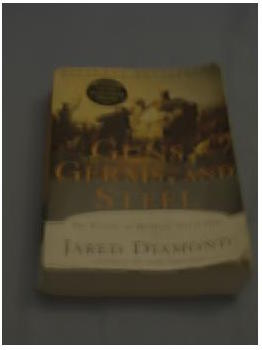
\includegraphics[width=1\linewidth]{book_deblurred} 
%\caption{Caption1}
%\label{fig:subim1}
%\end{wrapfigure}




\begin{figure*}
\begin{center}
\graphicspath{ {deblursun/} }
\begin{subfigure}{0.32\textwidth}

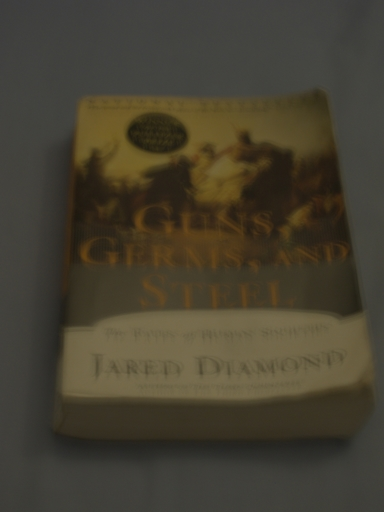
\includegraphics[width=0.9\linewidth]{book_s01_it0000_blurry} 
\caption{Blurry book image}
\label{fig:subim1}
\end{subfigure}
\begin{subfigure}{0.33\textwidth}
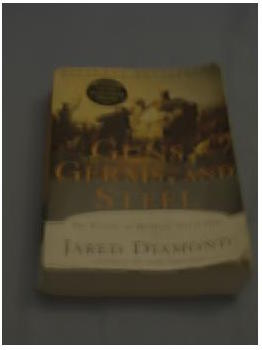
\includegraphics[width=0.9\linewidth]{book_deblurred}
\caption{Sun \etal (2015) result}
\label{fig:subim2}
\end{subfigure}
\begin{subfigure}{0.33\textwidth}
\graphicspath{ {deblurwhyte/} }
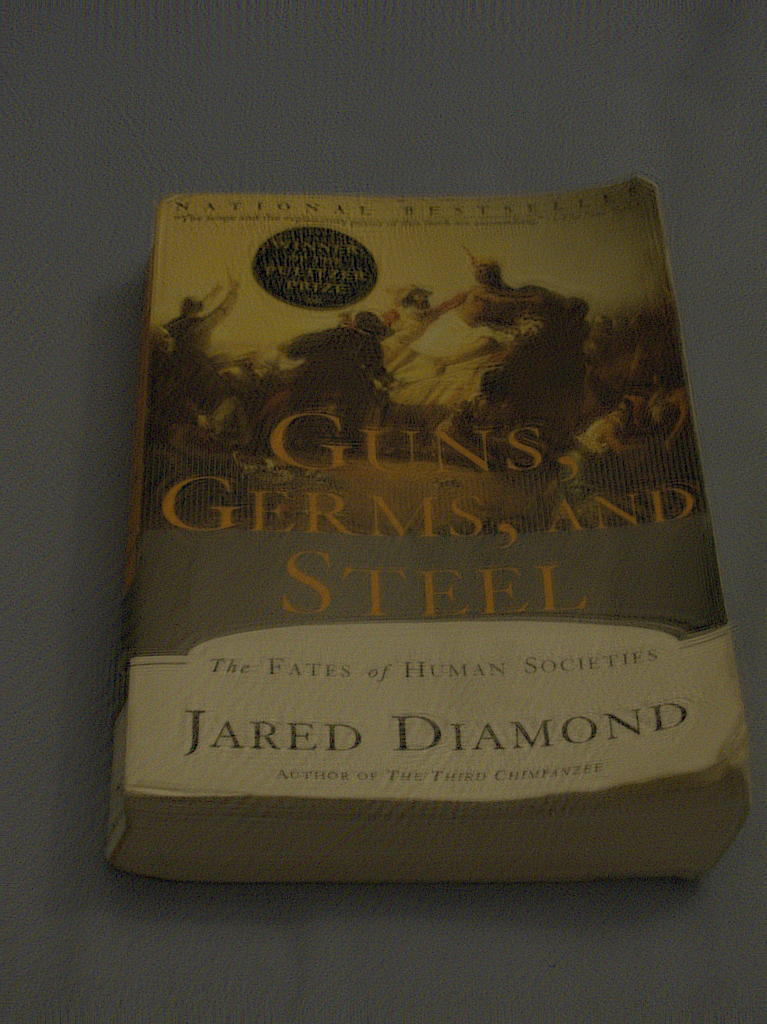
\includegraphics[width=0.9\linewidth]{book_whyte}
\caption{Whyte \etal (2012) result}
\label{fig:subim3}
\end{subfigure}
 
\caption{Blurry book image and deblurring results of the two algorithms}
\label{fig:image2}
\end{center}
\end{figure*}

%\begin{figure*}
%\begin{center}
%\graphicspath{ {deblursun/} }
%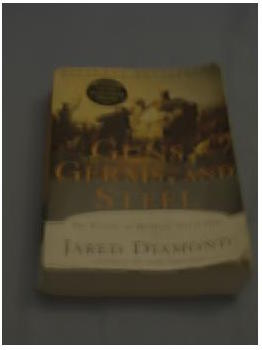
\includegraphics[width=0.4\linewidth]{book_deblurred}
%\caption{A caption}
%\end{center}
%\end{figure*}


\section{Conclusions}
In this study, we analyzed and evaluated two of the deblurring studies in the current literature. We evaluated the results using a recently developed metric that was designed to measure motion deblurring specifically. The results show that neither of the techniques is the panacea of the blind motion deblurring problem. Both techniques are good for certain types of blurry pictures.


%-------------------------------------------------------------------------

\subsection{Paper length}
Papers, excluding the references section,
must be no longer than eight pages in length. The references section
will not be included in the page count, and there is no limit on the
length of the references section. For example, a paper of eight pages
with two pages of references would have a total length of 10 pages.
{\bf There will be no extra page charges for
  CVPR 2016.}

%-------------------------------------------------------------------------
\subsection{The ruler}
The \LaTeX\ style defines a printed ruler which should be present in the
version submitted for review.  The ruler is provided in order that
reviewers may comment on particular lines in the paper without
circumlocution.  If you are preparing a document using a non-\LaTeX\
document preparation system, please arrange for an equivalent ruler to
appear on the final output pages.  The presence or absence of the ruler
should not change the appearance of any other content on the page.  The
camera ready copy should not contain a ruler. (\LaTeX\ users may uncomment
the \verb'\cvprfinalcopy' command in the document preamble.)  Reviewers:
note that the ruler measurements do not align well with lines in the paper
--- this turns out to be very difficult to do well when the paper contains
many figures and equations, and, when done, looks ugly.  Just use fractional
references (e.g.\ this line is $095.5$), although in most cases one would
expect that the approximate location will be adequate.

\subsection{Mathematics}

Please number all of your sections and displayed equations.  It is
important for readers to be able to refer to any particular equation.  Just
because you didn't refer to it in the text doesn't mean some future reader
might not need to refer to it.  It is cumbersome to have to use
circumlocutions like ``the equation second from the top of page 3 column
1''.  (Note that the ruler will not be present in the final copy, so is not
an alternative to equation numbers).  All authors will benefit from reading
Mermin's description of how to write mathematics:
\url{http://www.pamitc.org/documents/mermin.pdf}.


\subsection{Blind review}

Many authors misunderstand the concept of anonymizing for blind
review.  Blind review does not mean that one must remove
citations to one's own work---in fact it is often impossible to
review a paper unless the previous citations are known and
available.

Blind review means that you do not use the words ``my'' or ``our''
when citing previous work.  That is all.  (But see below for
techreports.)

Saying ``this builds on the work of Lucy Smith [1]'' does not say
that you are Lucy Smith; it says that you are building on her
work.  If you are Smith and Jones, do not say ``as we show in
[7]'', say ``as Smith and Jones show in [7]'' and at the end of the
paper, include reference 7 as you would any other cited work.

An example of a bad paper just asking to be rejected:
\begin{quote}
\begin{center}
    An analysis of the frobnicatable foo filter.
\end{center}

   In this paper we present a performance analysis of our
   previous paper [1], and show it to be inferior to all
   previously known methods.  Why the previous paper was
   accepted without this analysis is beyond me.

   [1] Removed for blind review
\end{quote}


An example of an acceptable paper:

\begin{quote}
\begin{center}
     An analysis of the frobnicatable foo filter.
\end{center}

   In this paper we present a performance analysis of the
   paper of Smith \etal [1], and show it to be inferior to
   all previously known methods.  Why the previous paper
   was accepted without this analysis is beyond me.

   [1] Smith, L and Jones, C. ``The frobnicatable foo
   filter, a fundamental contribution to human knowledge''.
   Nature 381(12), 1-213.
\end{quote}

If you are making a submission to another conference at the same time,
which covers similar or overlapping material, you may need to refer to that
submission in order to explain the differences, just as you would if you
had previously published related work.  In such cases, include the
anonymized parallel submission~\cite{Authors14} as additional material and
cite it as
\begin{quote}
[1] Authors. ``The frobnicatable foo filter'', F\&G 2014 Submission ID 324,
Supplied as additional material {\tt fg324.pdf}.
\end{quote}

Finally, you may feel you need to tell the reader that more details can be
found elsewhere, and refer them to a technical report.  For conference
submissions, the paper must stand on its own, and not {\em require} the
reviewer to go to a techreport for further details.  Thus, you may say in
the body of the paper ``further details may be found
in~\cite{Authors14b}''.  Then submit the techreport as additional material.
Again, you may not assume the reviewers will read this material. 

Sometimes your paper is about a problem which you tested using a tool which
is widely known to be restricted to a single institution.  For example,
let's say it's 1969, you have solved a key problem on the Apollo lander,
and you believe that the CVPR70 audience would like to hear about your
solution.  The work is a development of your celebrated 1968 paper entitled
``Zero-g frobnication: How being the only people in the world with access to
the Apollo lander source code makes us a wow at parties'', by Zeus \etal.

You can handle this paper like any other.  Don't write ``We show how to
improve our previous work [Anonymous, 1968].  This time we tested the
algorithm on a lunar lander [name of lander removed for blind review]''.
That would be silly, and would immediately identify the authors. Instead
write the following:
\begin{quotation}
\noindent
   We describe a system for zero-g frobnication.  This
   system is new because it handles the following cases:
   A, B.  Previous systems [Zeus et al. 1968] didn't
   handle case B properly.  Ours handles it by including
   a foo term in the bar integral.

   ...

   The proposed system was integrated with the Apollo
   lunar lander, and went all the way to the moon, don't
   you know.  It displayed the following behaviours
   which show how well we solved cases A and B: ...
\end{quotation}
As you can see, the above text follows standard scientific convention,
reads better than the first version, and does not explicitly name you as
the authors.  A reviewer might think it likely that the new paper was
written by Zeus \etal, but cannot make any decision based on that guess.
He or she would have to be sure that no other authors could have been
contracted to solve problem B.

FAQ: Are acknowledgements OK?  No.  Leave them for the final copy.


\begin{figure}[t]
\begin{center}
\fbox{\rule{0pt}{2in} \rule{0.9\linewidth}{0pt}}
   %\includegraphics[width=0.8\linewidth]{egfigure.eps}
\end{center}
   \caption{Example of caption.  It is set in Roman so that mathematics
   (always set in Roman: $B \sin A = A \sin B$) may be included without an
   ugly clash.}
\label{fig:long}
\label{fig:onecol}
\end{figure}

\subsection{Miscellaneous}

\noindent
Compare the following:\\
\begin{tabular}{ll}
 \verb'$conf_a$' &  $conf_a$ \\
 \verb'$\mathit{conf}_a$' & $\mathit{conf}_a$
\end{tabular}\\
See The \TeX book, p165.

The space after \eg, meaning ``for example'', should not be a
sentence-ending space. So \eg is correct, {\em e.g.} is not.  The provided
\verb'\eg' macro takes care of this.

When citing a multi-author paper, you may save space by using ``et alia'',
shortened to ``\etal'' (not ``{\em et.\ al.}'' as ``{\em et}'' is a complete word.)
However, use it only when there are three or more authors.  Thus, the
following is correct: ``
   Frobnication has been trendy lately.
   It was introduced by Alpher~\cite{Alpher02}, and subsequently developed by
   Alpher and Fotheringham-Smythe~\cite{Alpher03}, and Alpher \etal~\cite{Alpher04}.''

This is incorrect: ``... subsequently developed by Alpher \etal~\cite{Alpher03} ...''
because reference~\cite{Alpher03} has just two authors.  If you use the
\verb'\etal' macro provided, then you need not worry about double periods
when used at the end of a sentence as in Alpher \etal.

For this citation style, keep multiple citations in numerical (not
chronological) order, so prefer \cite{Alpher03,Alpher02,Authors14} to
\cite{Alpher02,Alpher03,Authors14}.


\begin{figure*}
\begin{center}
\fbox{\rule{0pt}{2in} \rule{.9\linewidth}{0pt}}
\end{center}
   \caption{Example of a short caption, which should be centered.}
\label{fig:short}
\end{figure*}

%------------------------------------------------------------------------
\section{Formatting your paper}

All text must be in a two-column format. The total allowable width of the
text area is $6\frac78$ inches (17.5 cm) wide by $8\frac78$ inches (22.54
cm) high. Columns are to be $3\frac14$ inches (8.25 cm) wide, with a
$\frac{5}{16}$ inch (0.8 cm) space between them. The main title (on the
first page) should begin 1.0 inch (2.54 cm) from the top edge of the
page. The second and following pages should begin 1.0 inch (2.54 cm) from
the top edge. On all pages, the bottom margin should be 1-1/8 inches (2.86
cm) from the bottom edge of the page for $8.5 \times 11$-inch paper; for A4
paper, approximately 1-5/8 inches (4.13 cm) from the bottom edge of the
page.

%-------------------------------------------------------------------------
\subsection{Margins and page numbering}

All printed material, including text, illustrations, and charts, must be kept
within a print area 6-7/8 inches (17.5 cm) wide by 8-7/8 inches (22.54 cm)
high.
Page numbers should be in footer with page numbers, centered and .75
inches from the bottom of the page and make it start at the correct page
number rather than the 4321 in the example.  To do this fine the line (around
line 23)
\begin{verbatim}
%\ifcvprfinal\pagestyle{empty}\fi
\setcounter{page}{1}
\end{verbatim}
where the number 4321 is your assigned starting page.

Make sure the first page is numbered by commenting out the first page being
empty on line 46
\begin{verbatim}
%\thispagestyle{empty}
\end{verbatim}


%-------------------------------------------------------------------------
\subsection{Type-style and fonts}

Wherever Times is specified, Times Roman may also be used. If neither is
available on your word processor, please use the font closest in
appearance to Times to which you have access.

MAIN TITLE. Center the title 1-3/8 inches (3.49 cm) from the top edge of
the first page. The title should be in Times 14-point, boldface type.
Capitalize the first letter of nouns, pronouns, verbs, adjectives, and
adverbs; do not capitalize articles, coordinate conjunctions, or
prepositions (unless the title begins with such a word). Leave two blank
lines after the title.

AUTHOR NAME(s) and AFFILIATION(s) are to be centered beneath the title
and printed in Times 12-point, non-boldface type. This information is to
be followed by two blank lines.

The ABSTRACT and MAIN TEXT are to be in a two-column format.

MAIN TEXT. Type main text in 10-point Times, single-spaced. Do NOT use
double-spacing. All paragraphs should be indented 1 pica (approx. 1/6
inch or 0.422 cm). Make sure your text is fully justified---that is,
flush left and flush right. Please do not place any additional blank
lines between paragraphs.

Figure and table captions should be 9-point Roman type as in
Figures~\ref{fig:onecol} and~\ref{fig:short}.  Short captions should be centred.

\noindent Callouts should be 9-point Helvetica, non-boldface type.
Initially capitalize only the first word of section titles and first-,
second-, and third-order headings.

FIRST-ORDER HEADINGS. (For example, {\large \bf 1. Introduction})
should be Times 12-point boldface, initially capitalized, flush left,
with one blank line before, and one blank line after.

SECOND-ORDER HEADINGS. (For example, { \bf 1.1. Database elements})
should be Times 11-point boldface, initially capitalized, flush left,
with one blank line before, and one after. If you require a third-order
heading (we discourage it), use 10-point Times, boldface, initially
capitalized, flush left, preceded by one blank line, followed by a period
and your text on the same line.

%-------------------------------------------------------------------------
\subsection{Footnotes}

Please use footnotes\footnote {This is what a footnote looks like.  It
often distracts the reader from the main flow of the argument.} sparingly.
Indeed, try to avoid footnotes altogether and include necessary peripheral
observations in
the text (within parentheses, if you prefer, as in this sentence).  If you
wish to use a footnote, place it at the bottom of the column on the page on
which it is referenced. Use Times 8-point type, single-spaced.


%-------------------------------------------------------------------------
\subsection{References}

List and number all bibliographical references in 9-point Times,
single-spaced, at the end of your paper. When referenced in the text,
enclose the citation number in square brackets, for
example~\cite{Authors14}.  Where appropriate, include the name(s) of
editors of referenced books.

\begin{table}
\begin{center}
\begin{tabular}{|l|c|}
\hline
Method & Frobnability \\
\hline\hline
Theirs & Frumpy \\
Yours & Frobbly \\
Ours & Makes one's heart Frob\\
\hline
\end{tabular}
\end{center}
\caption{Results.   Ours is better.}
\end{table}

%-------------------------------------------------------------------------
\subsection{Illustrations, graphs, and photographs}

All graphics should be centered.  Please ensure that any point you wish to
make is resolvable in a printed copy of the paper.  Resize fonts in figures
to match the font in the body text, and choose line widths which render
effectively in print.  Many readers (and reviewers), even of an electronic
copy, will choose to print your paper in order to read it.  You cannot
insist that they do otherwise, and therefore must not assume that they can
zoom in to see tiny details on a graphic.

When placing figures in \LaTeX, it's almost always best to use
\verb+\includegraphics+, and to specify the  figure width as a multiple of
the line width as in the example below
{\small\begin{verbatim}
   \usepackage[dvips]{graphicx} ...
   \includegraphics[width=0.8\linewidth]
                   {myfile.eps}
\end{verbatim}
}


%-------------------------------------------------------------------------
\subsection{Color}

Please refer to the author guidelines on the CVPR 2016 web page for a discussion
of the use of color in your document.

%------------------------------------------------------------------------
\section{Final copy}

You must include your signed IEEE copyright release form when you submit
your finished paper. We MUST have this form before your paper can be
published in the proceedings.


{\small
\bibliographystyle{ieee}
\bibliography{egbib}
}

\end{document}
